\chapter*{Annexes}
\addcontentsline{toc}{chapter}{Annexes}

\section*{Chapitre 4}

\newpage
\subsection*{Analyse détaillée des variables (sortie complète de l'agent)}

\newsavebox{\tempimage}
\sbox{\tempimage}{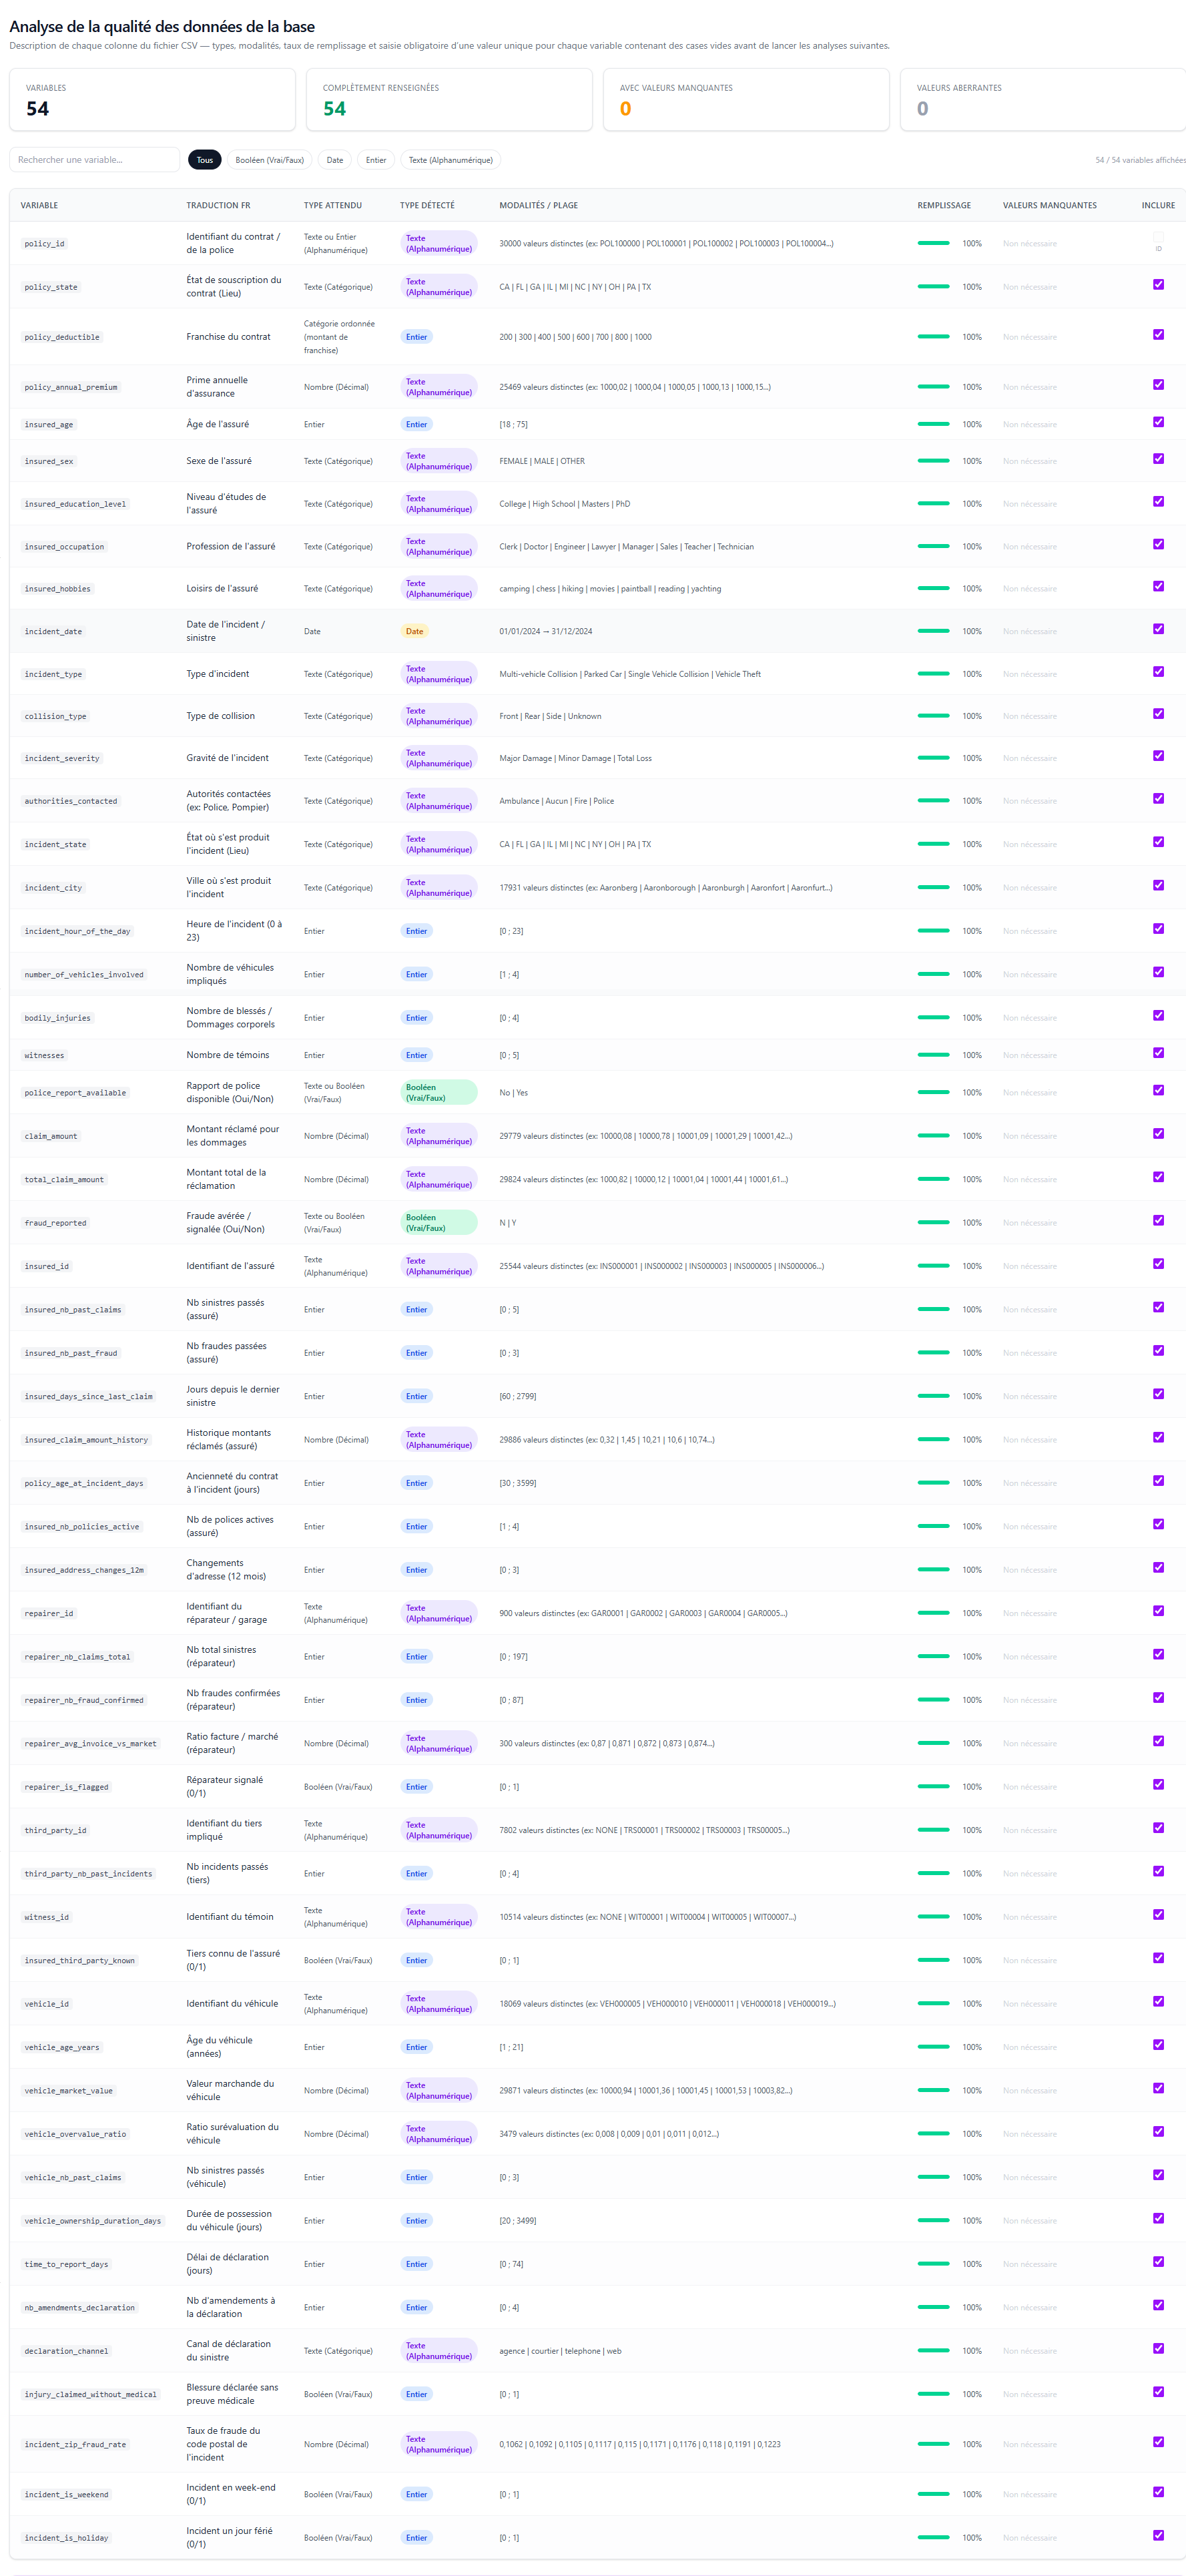
\includegraphics[width=\textwidth]{images/annexe/analyse_variables.png}}

% ---  1 / 5 (lignes du haut : coupe 80% en bas) ---
\begin{center}
    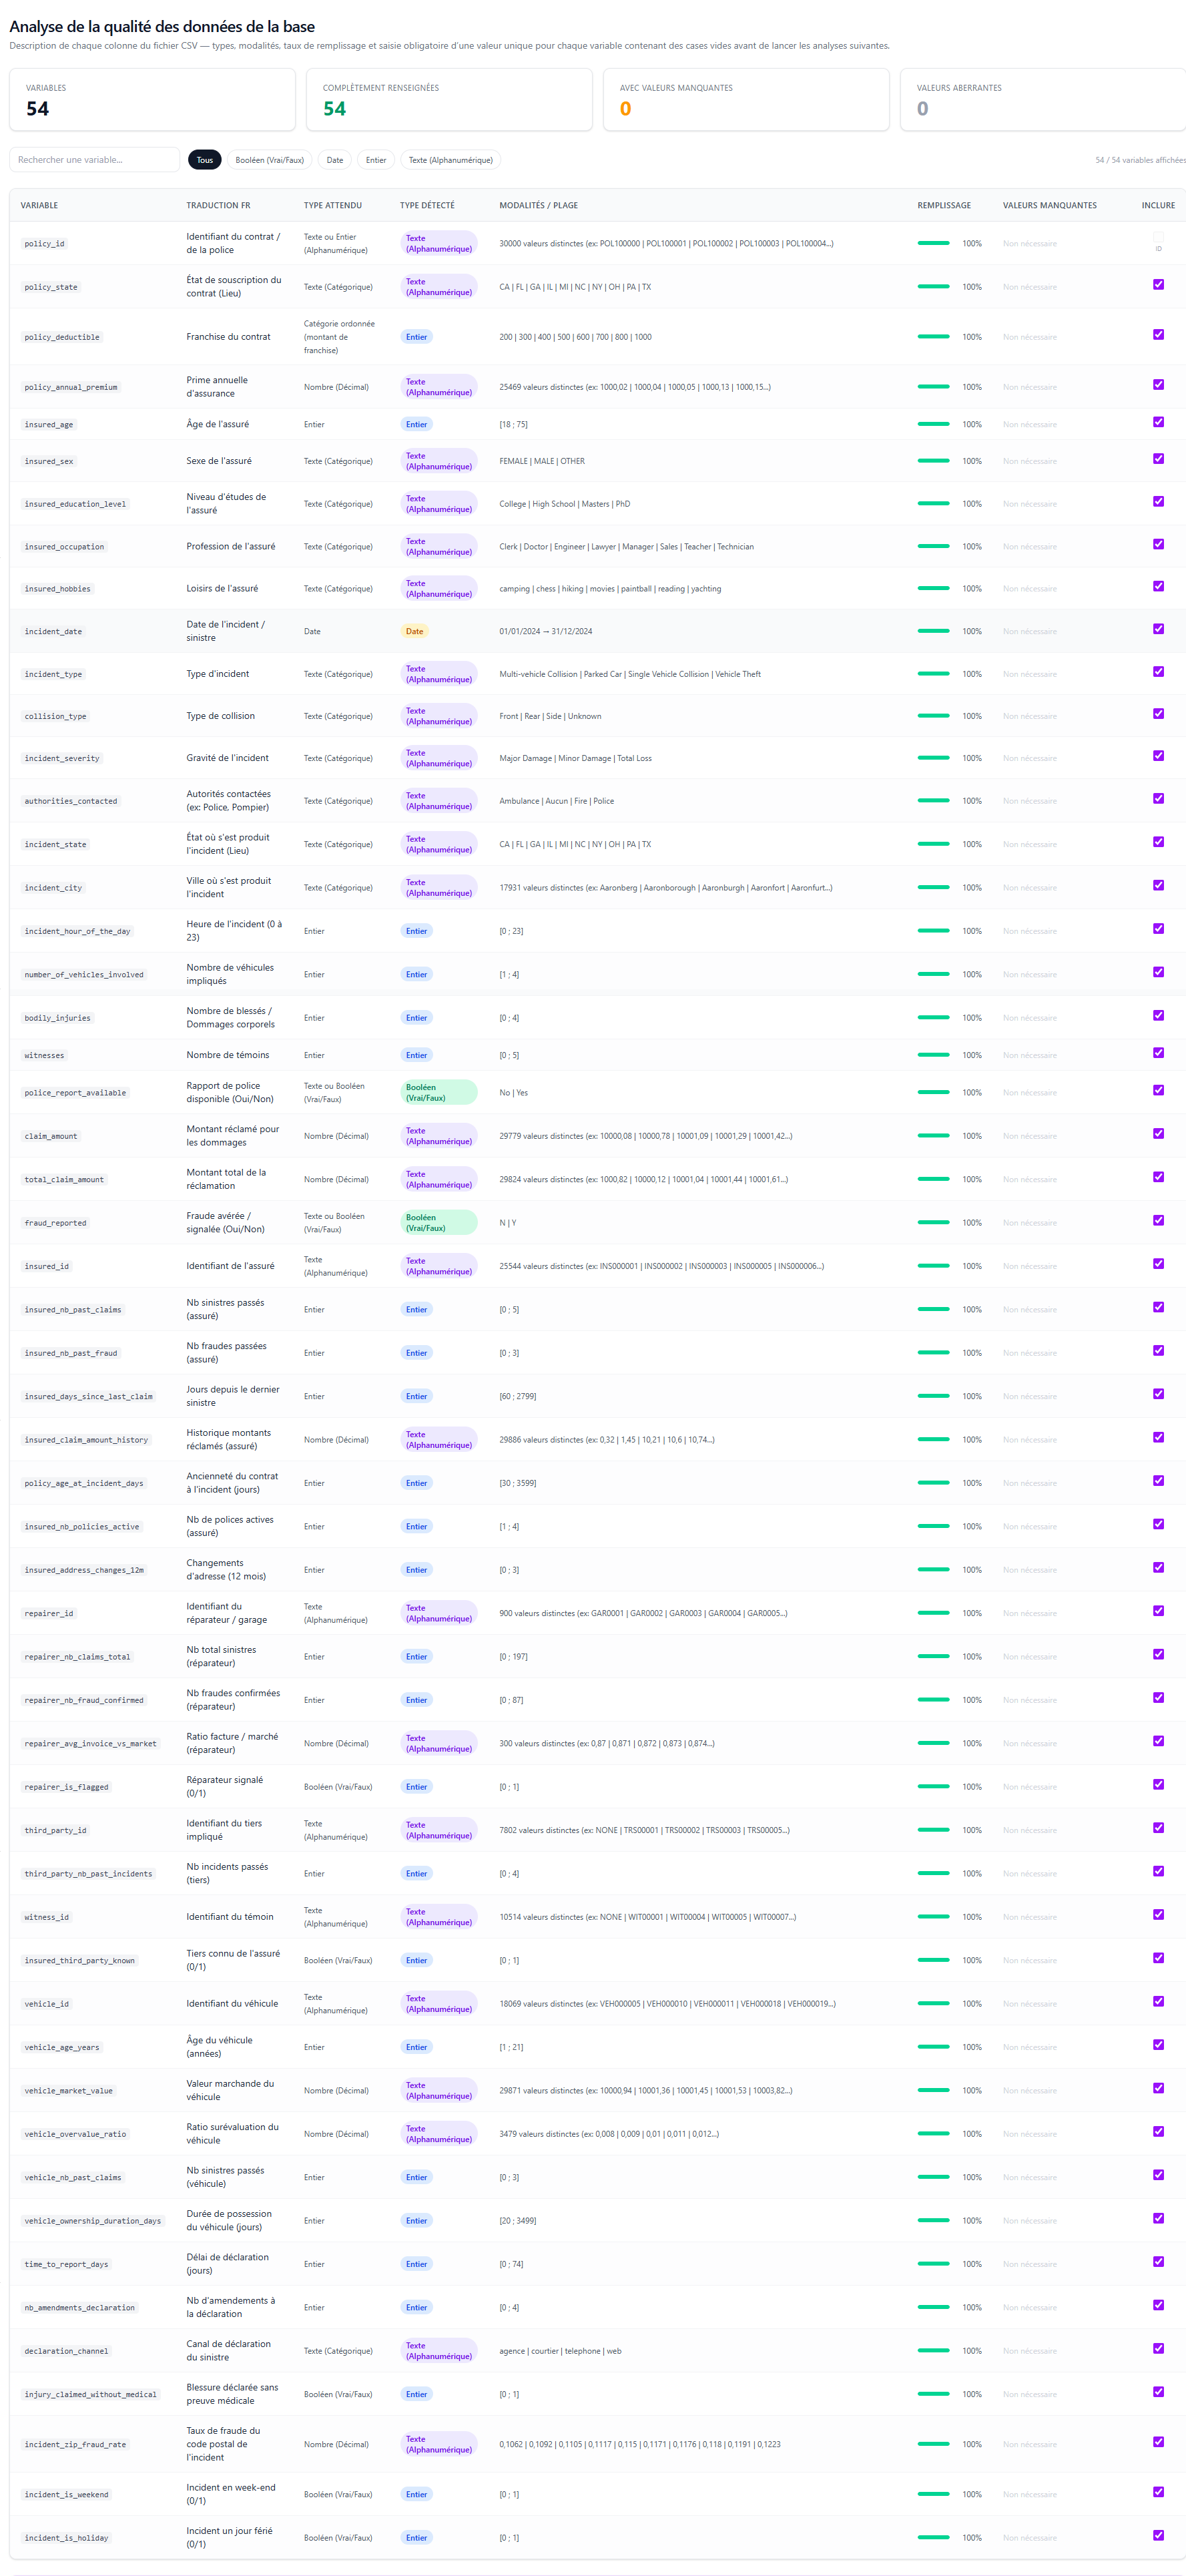
\includegraphics[width=\textwidth,trim=0pt {\dimexpr0.8\ht\tempimage} 0pt 0pt,clip]{images/annexe/analyse_variables.png}
\end{center}

\clearpage

% ---  2 / 5 (coupe 20% en haut et 60% en bas) ---
\begin{center}
    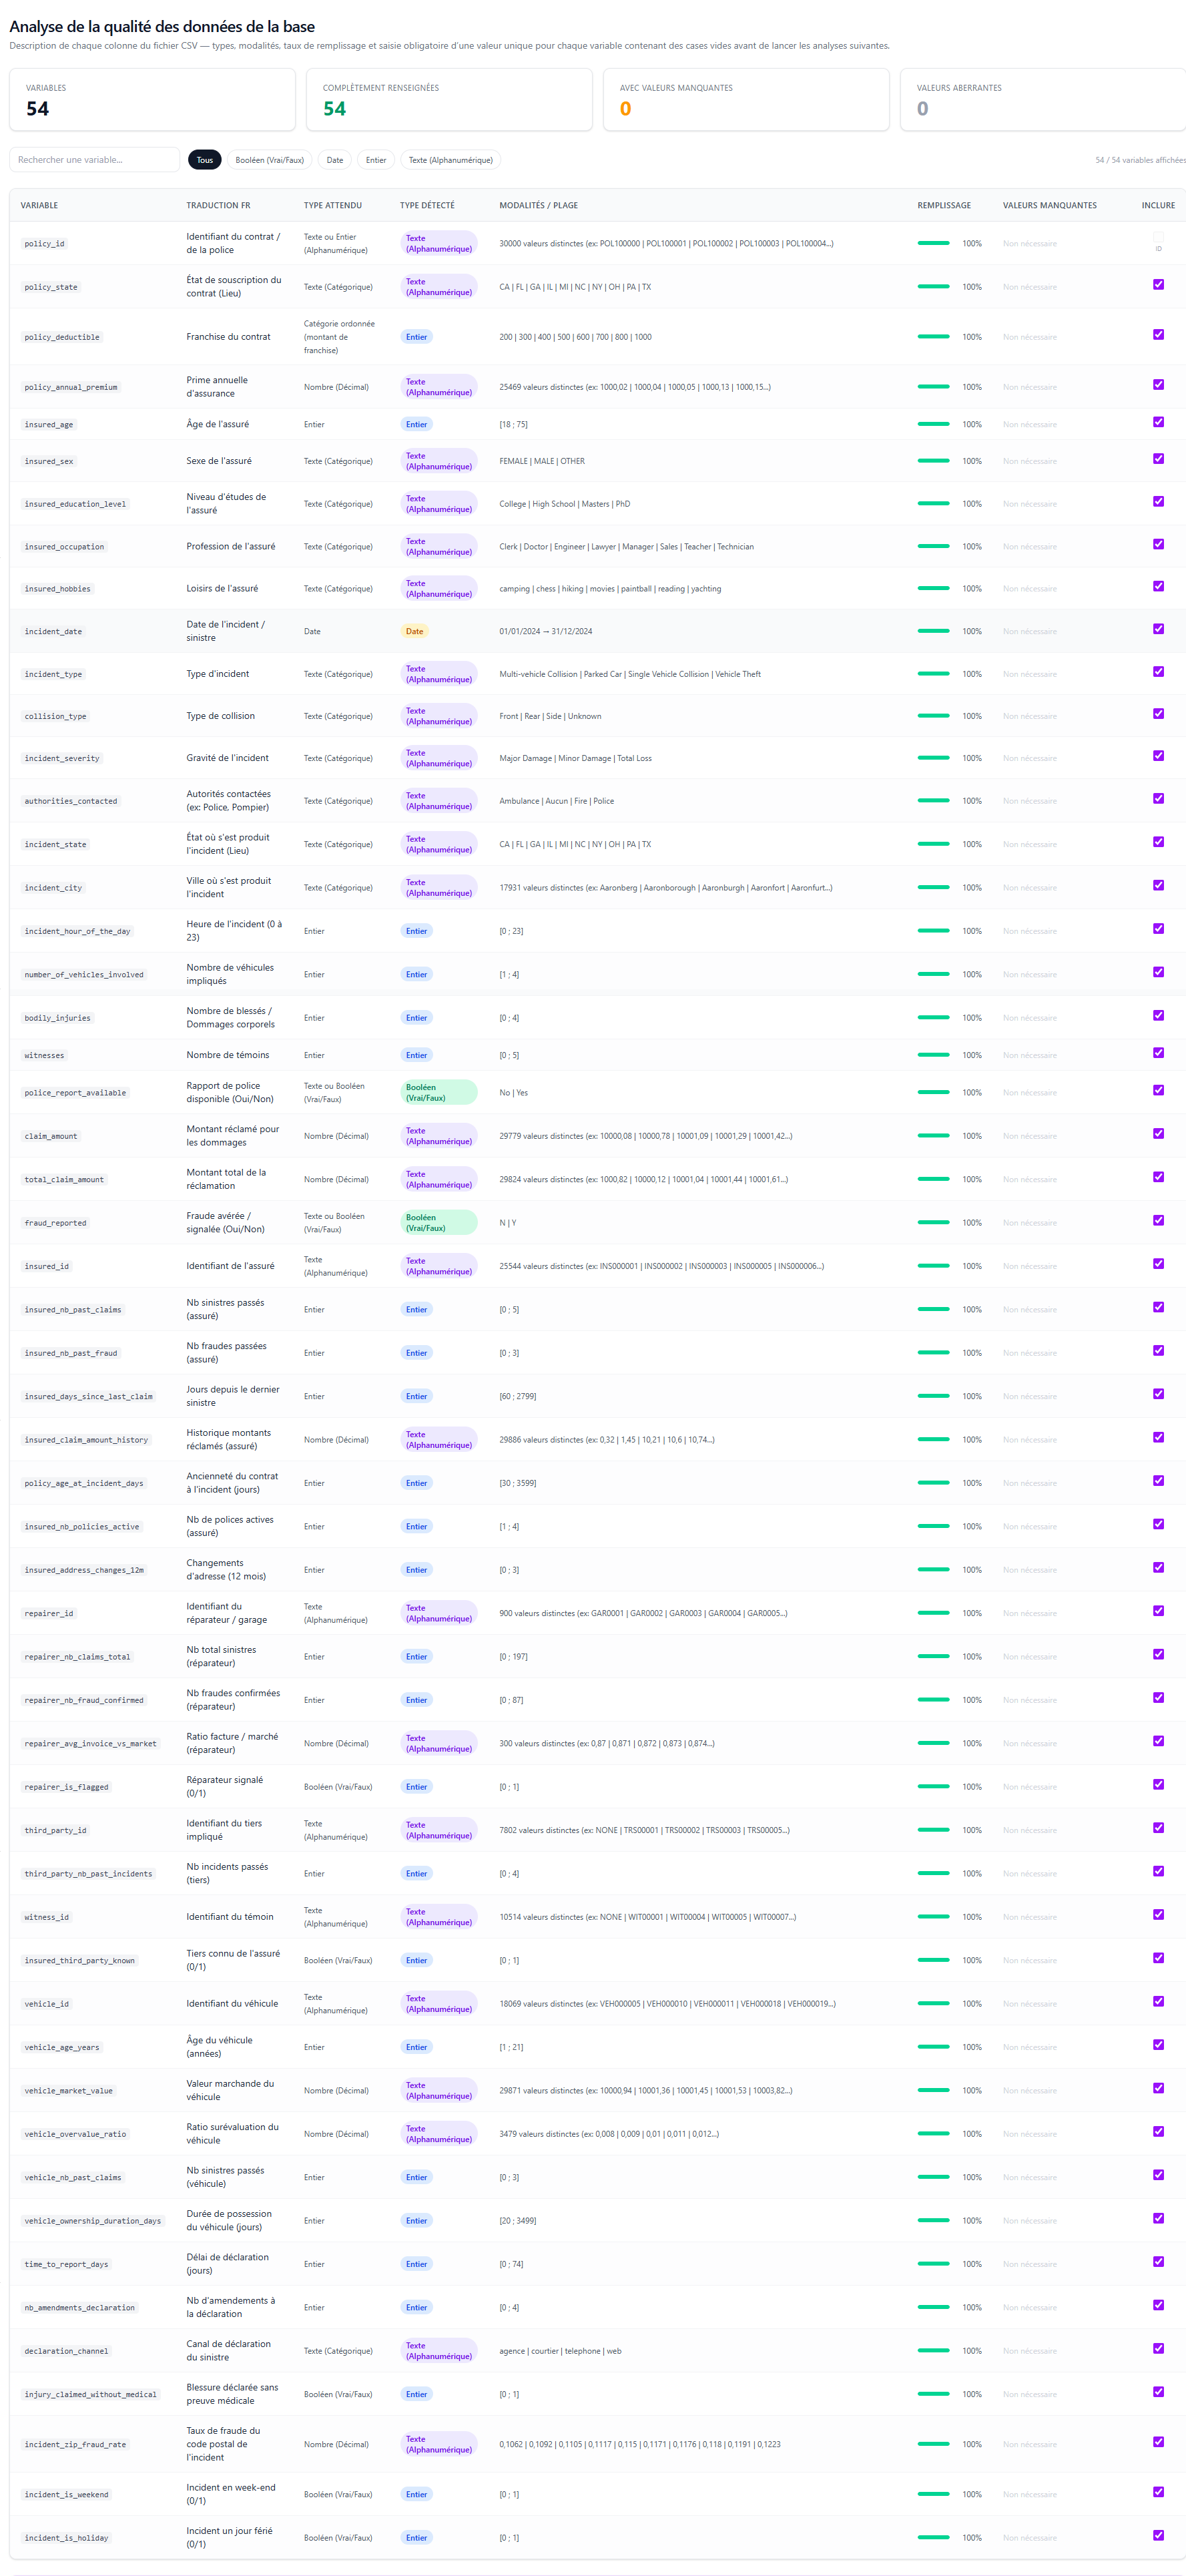
\includegraphics[width=\textwidth,trim=0pt {\dimexpr0.60\ht\tempimage} 0pt {\dimexpr0.20\ht\tempimage},clip]{images/annexe/analyse_variables.png}
\end{center}

\clearpage

% ---  3 / 5 (coupe 40% en haut et 40% en bas) ---
\begin{center}
    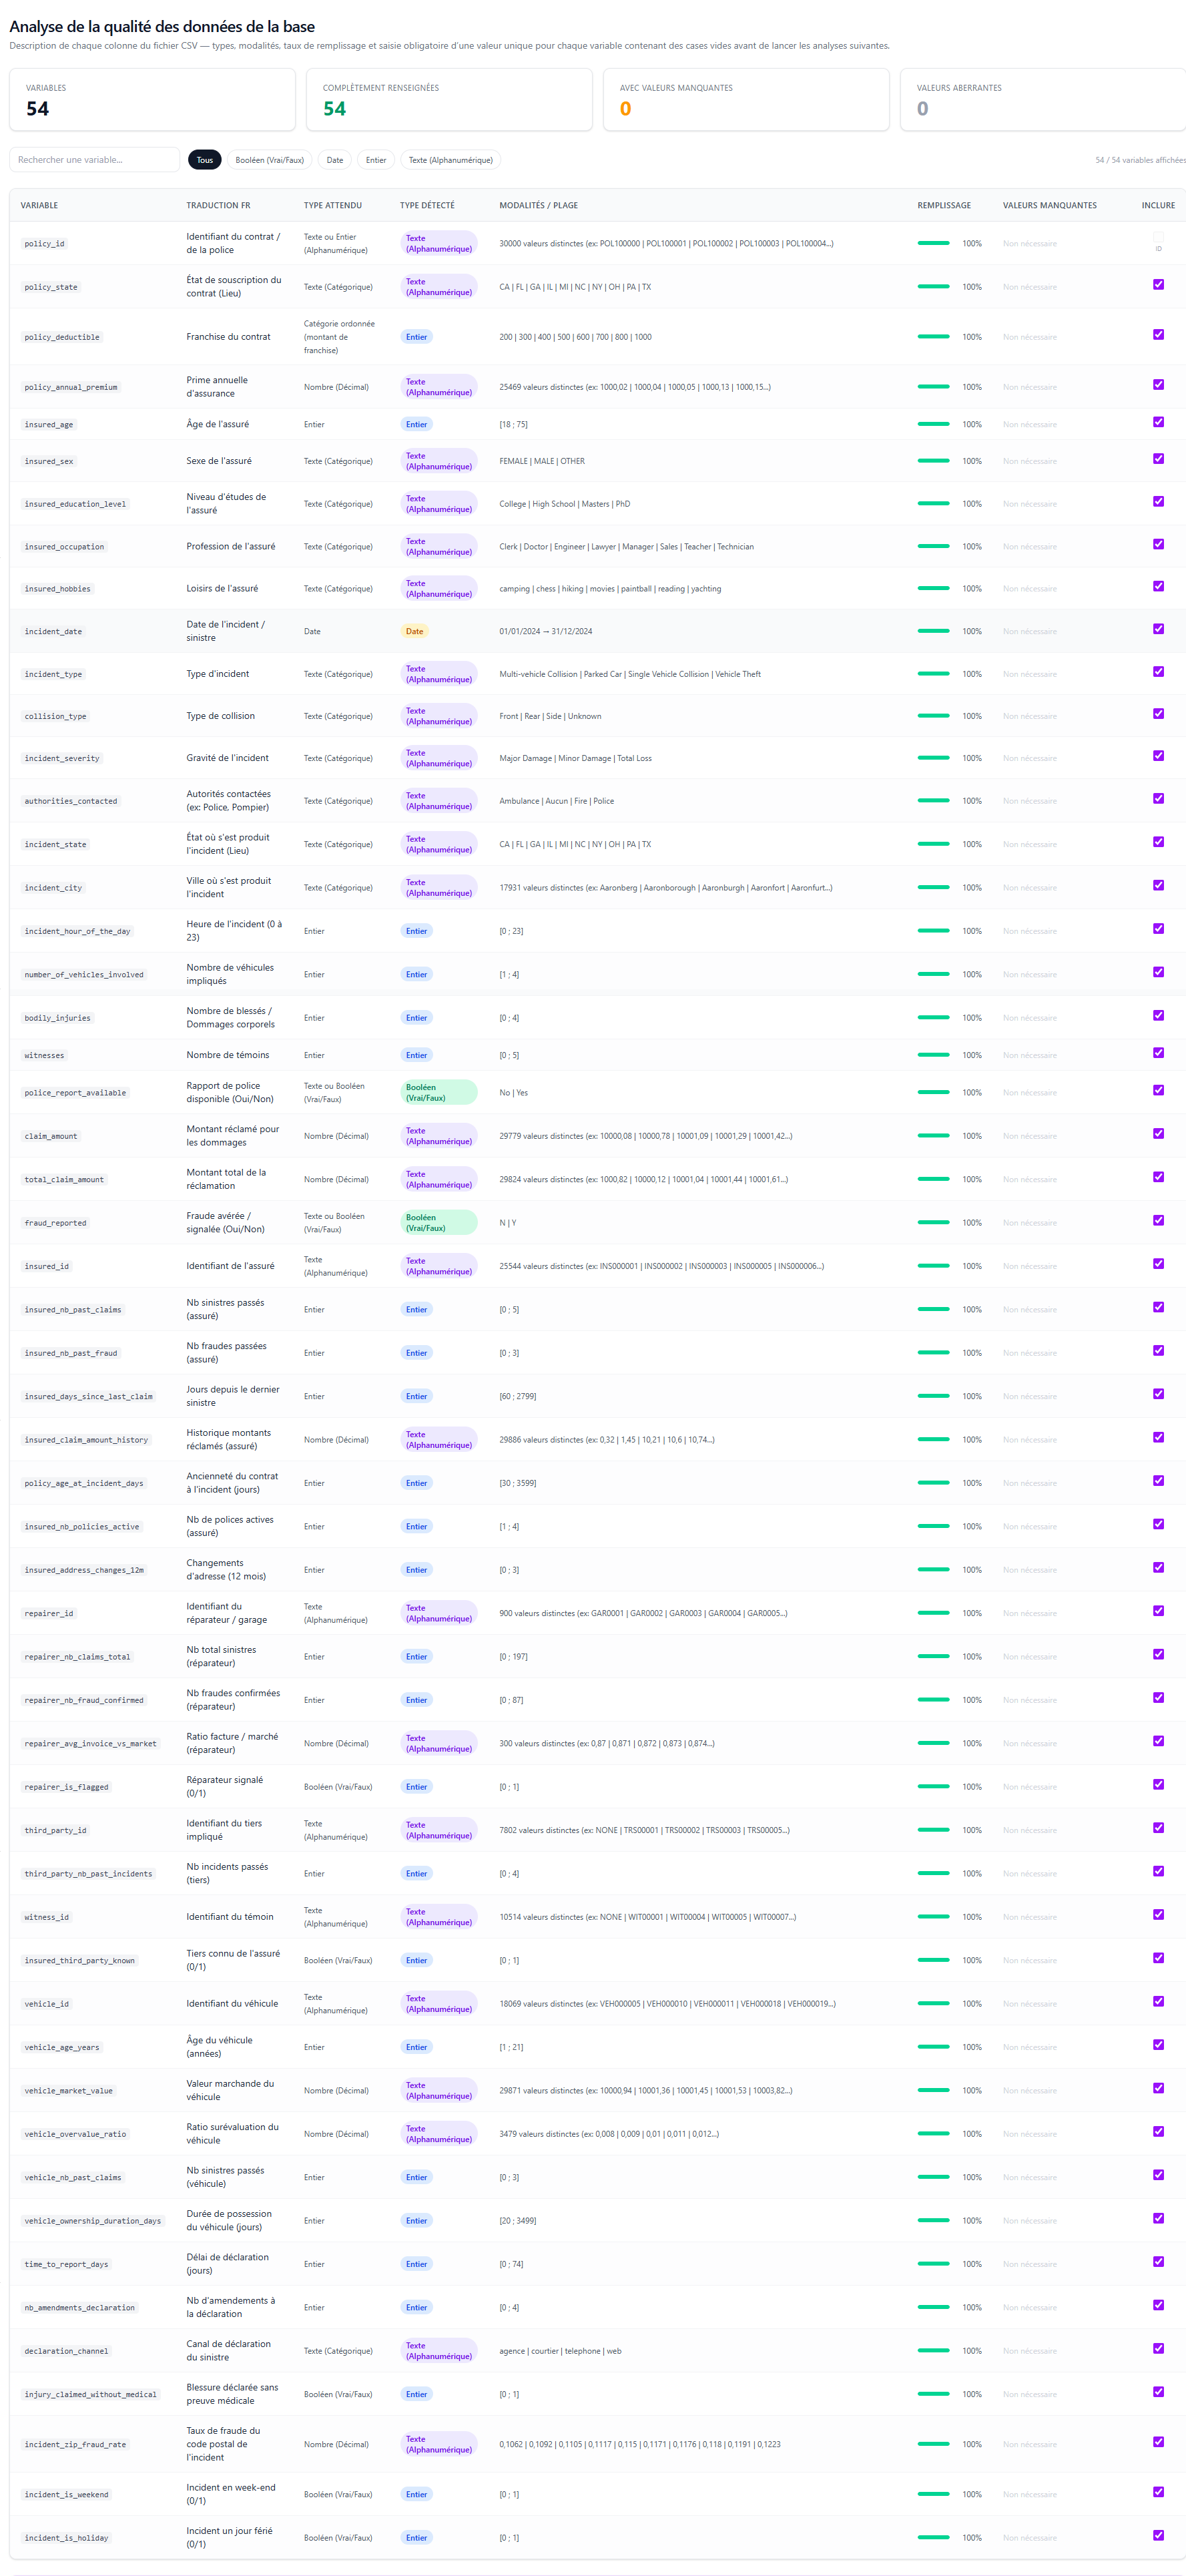
\includegraphics[width=\textwidth,trim=0pt {\dimexpr0.40\ht\tempimage} 0pt {\dimexpr0.40\ht\tempimage},clip]{images/annexe/analyse_variables.png}
\end{center}

\clearpage

% ---  4 / 5 (coupe 60% en haut et 20% en bas) ---
\begin{center}
    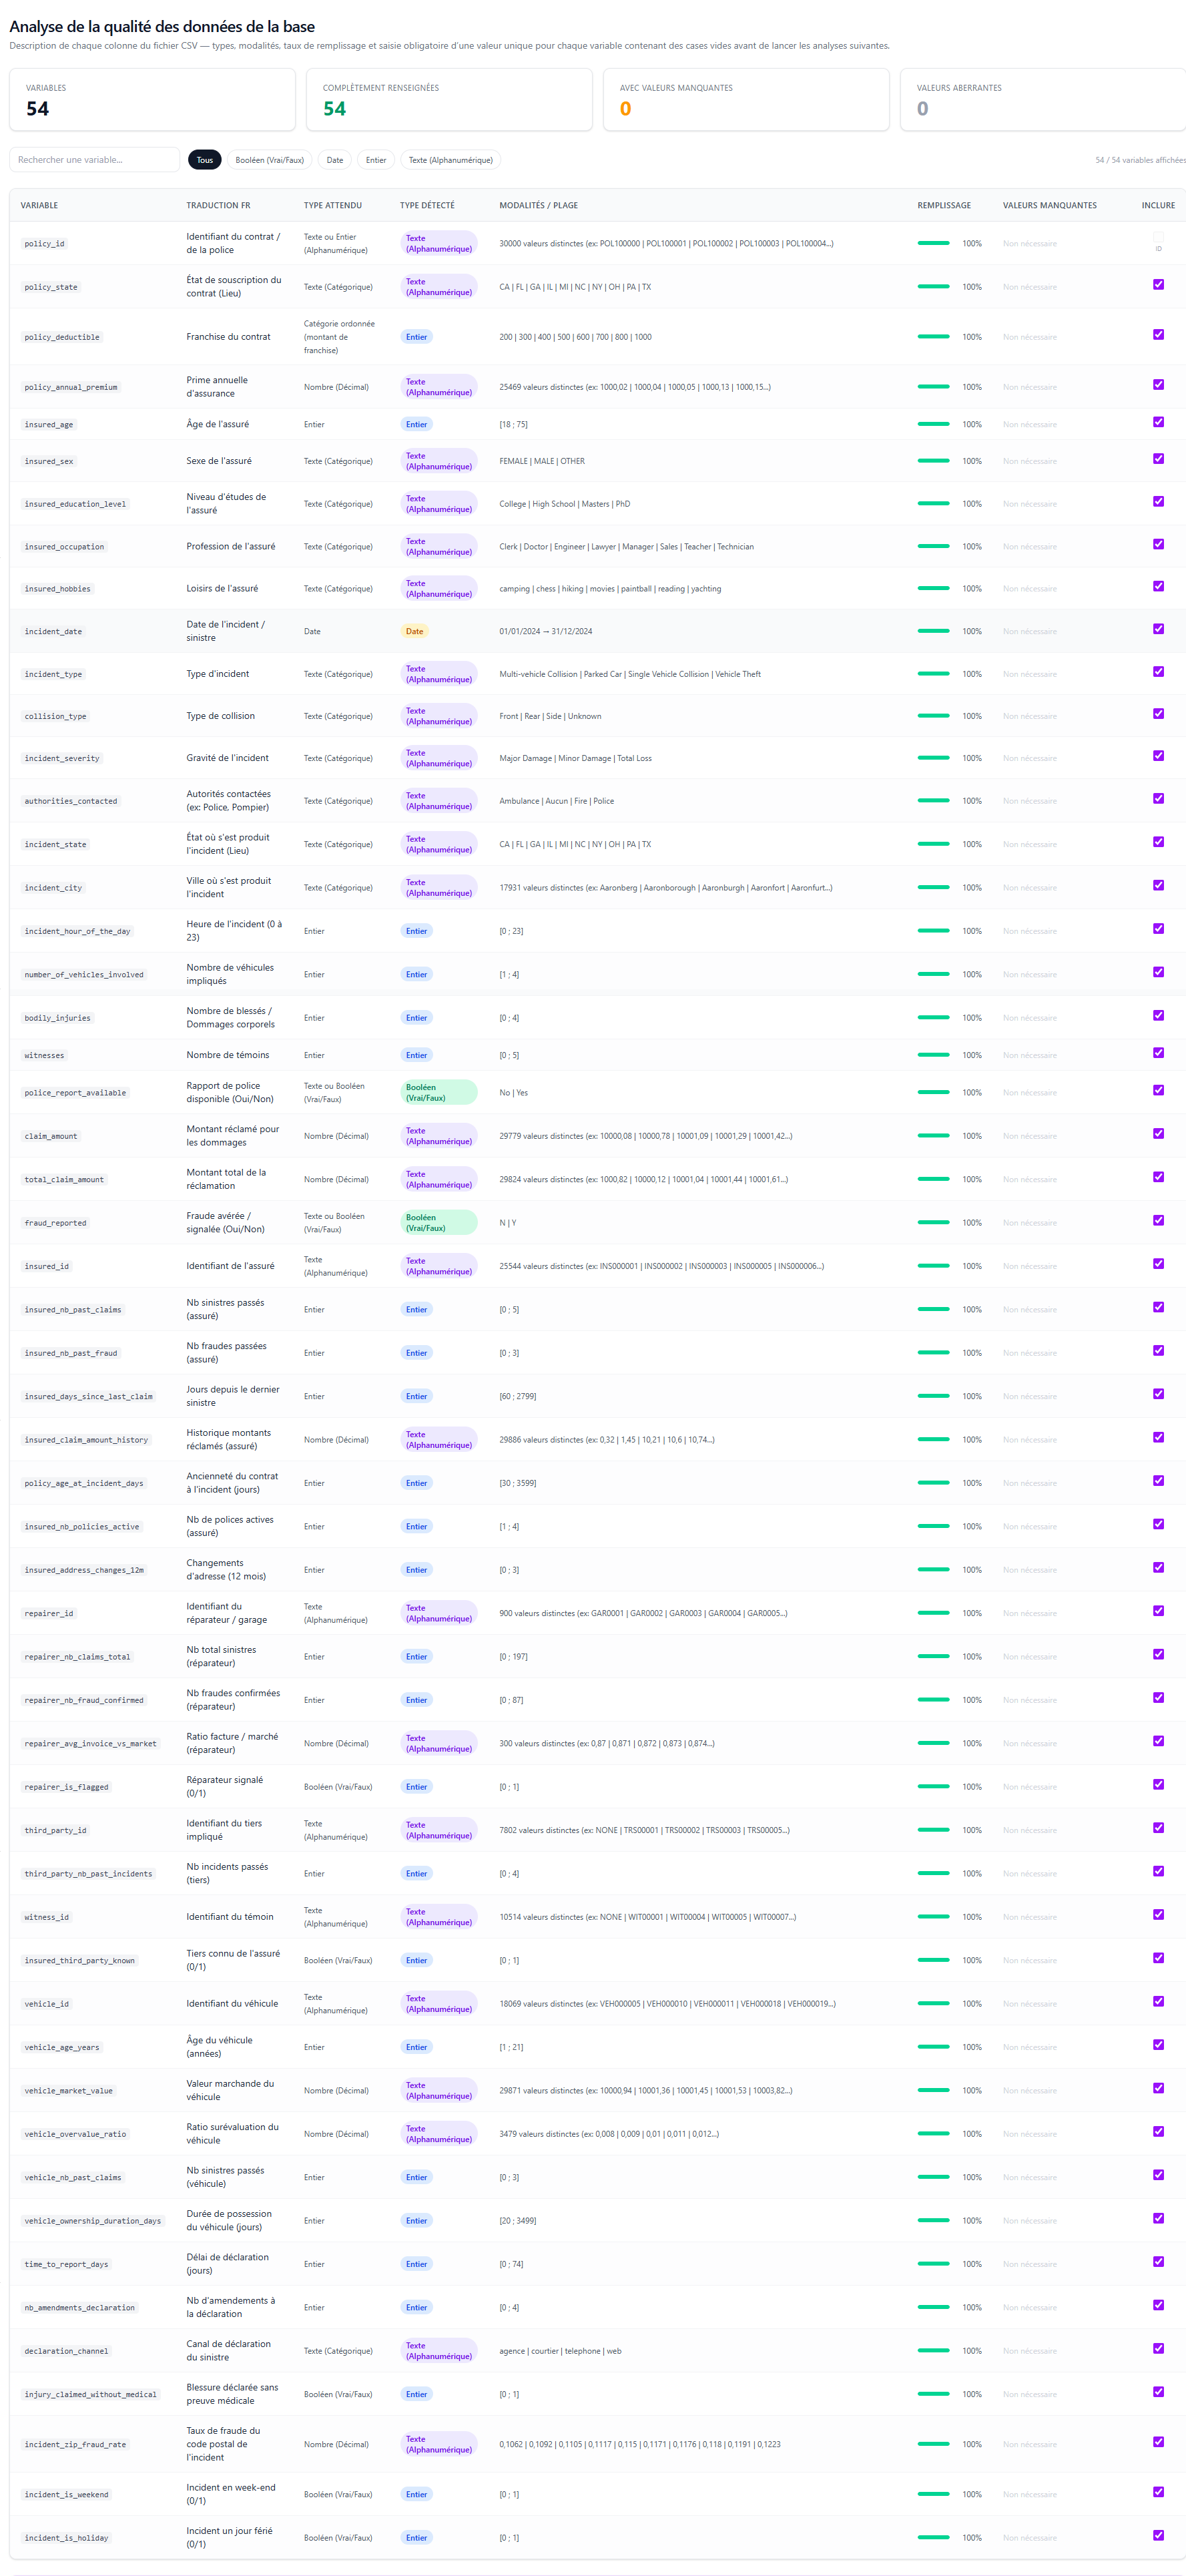
\includegraphics[width=\textwidth,trim=0pt {\dimexpr0.2\ht\tempimage} 0pt {\dimexpr0.60\ht\tempimage},clip]{images/annexe/analyse_variables.png}
\end{center}


% ---  5 / 5 (lignes du bas : coupe 80% en haut) ---
\begin{center}
    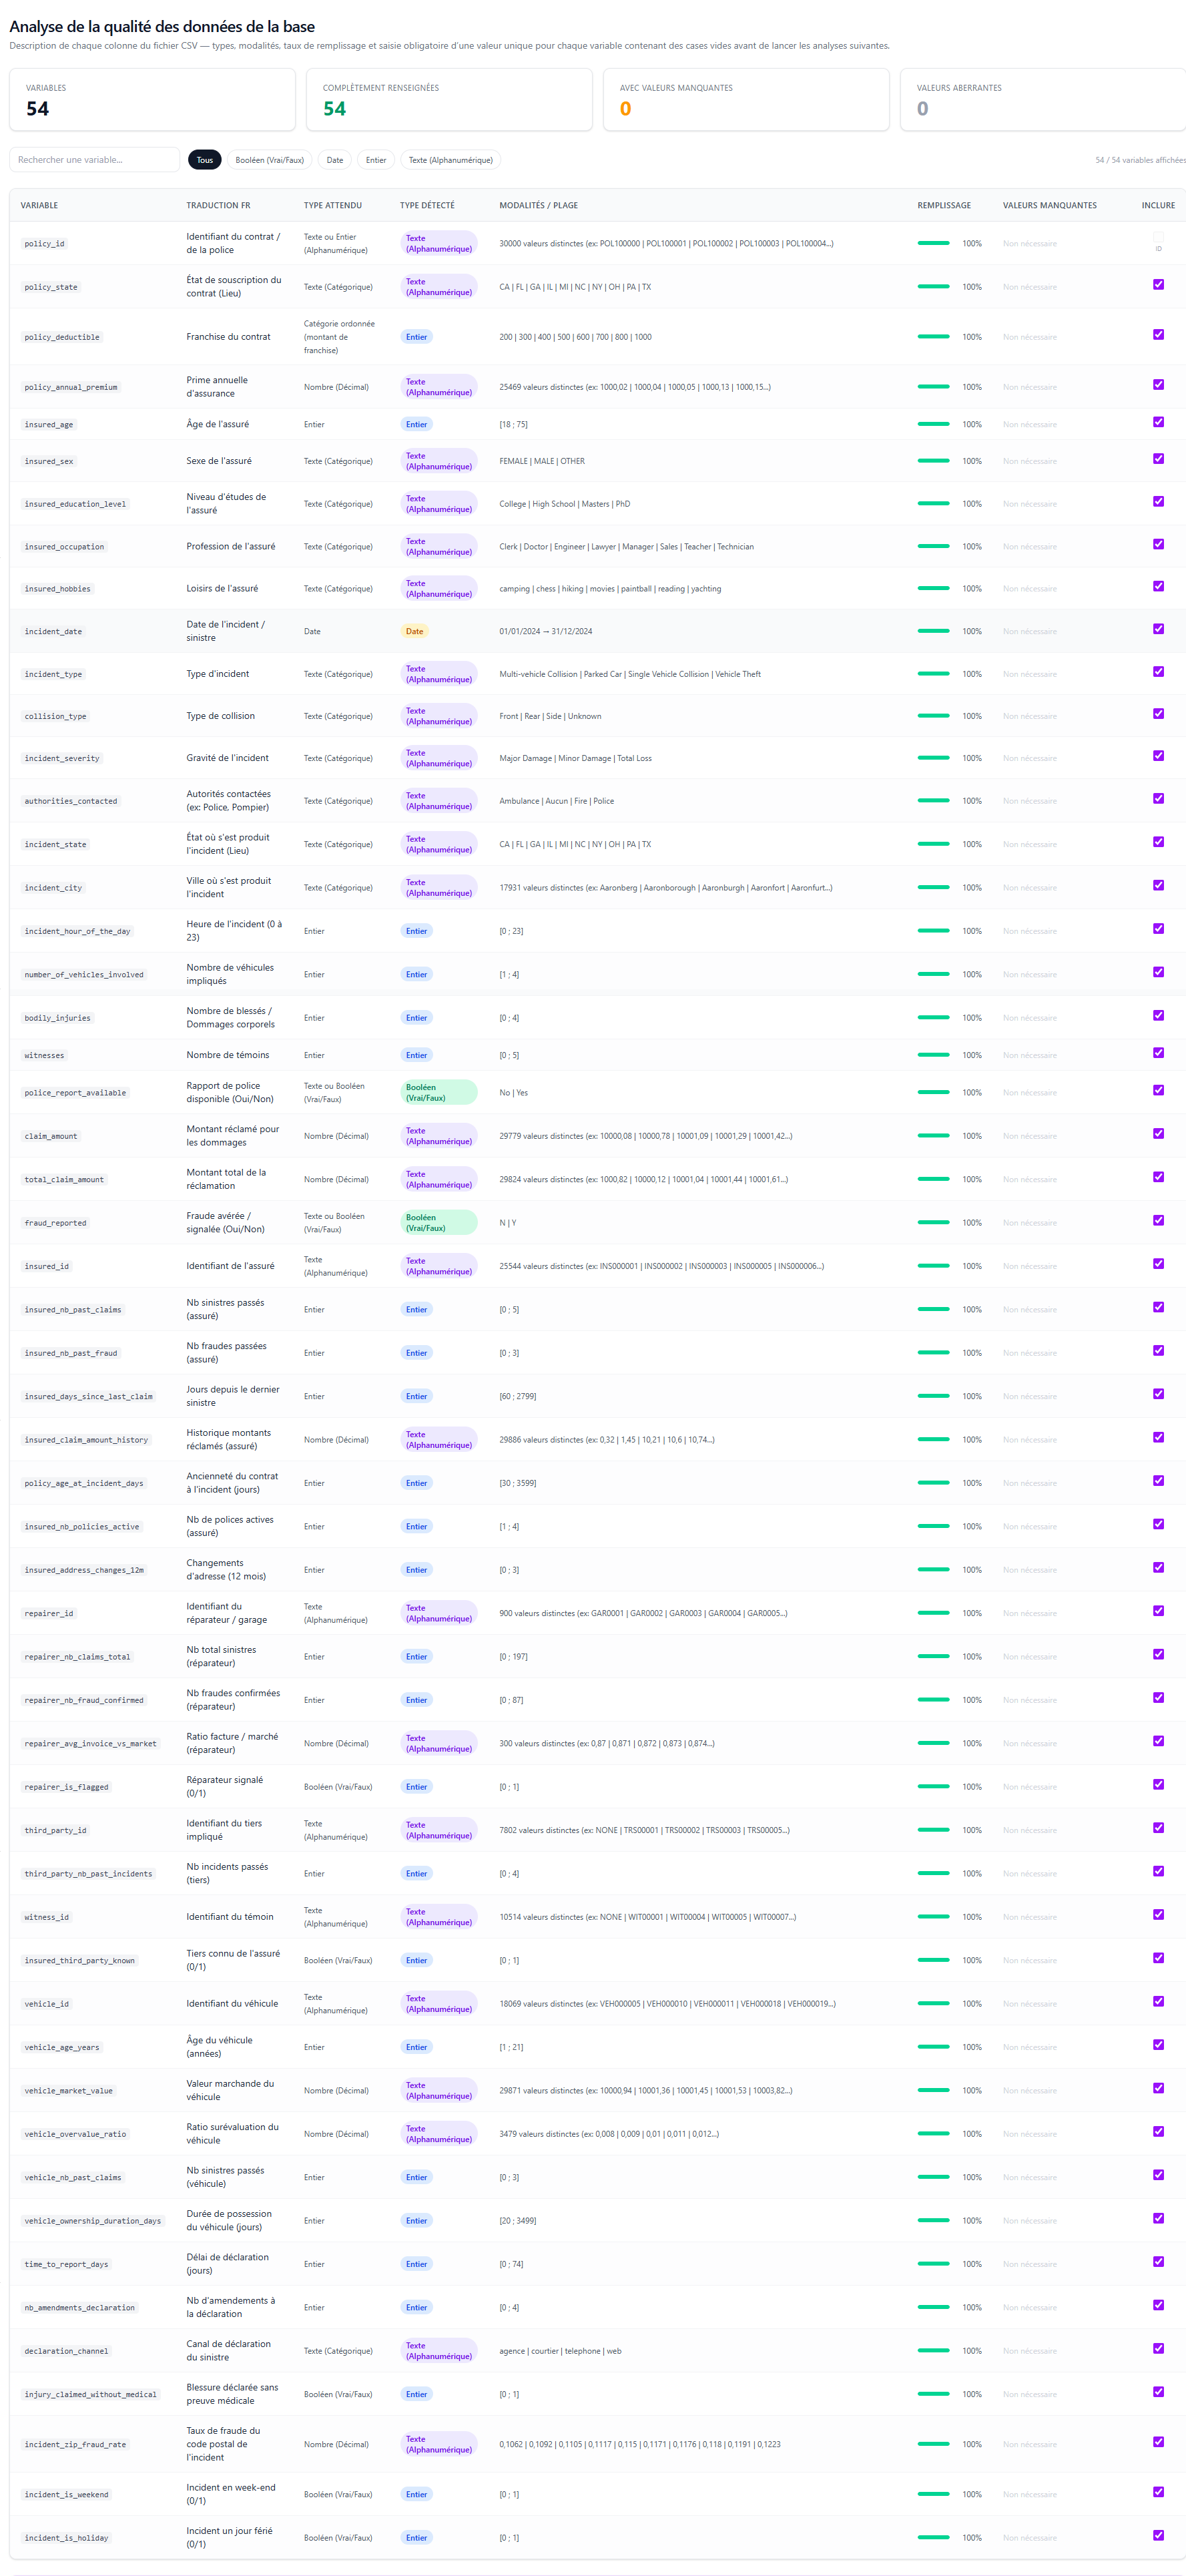
\includegraphics[width=\textwidth,trim=0pt 0pt 0pt {\dimexpr0.8\ht\tempimage},clip]{images/annexe/analyse_variables.png}
\end{center}




\clearpage

\subsection*{Analyse des variables selon le statut de fraude (sortie complète de l'agent)}

\begin{center}
    
\includegraphics[width=\textwidth,height=0.85\textheight,keepaspectratio]{images/annexe/analyse_variables_selon_fraude.png}
\end{center}

\clearpage

\subsection*{Composition détaillée du portefeuille (sortie complète de l'agent)}

\begin{center}
    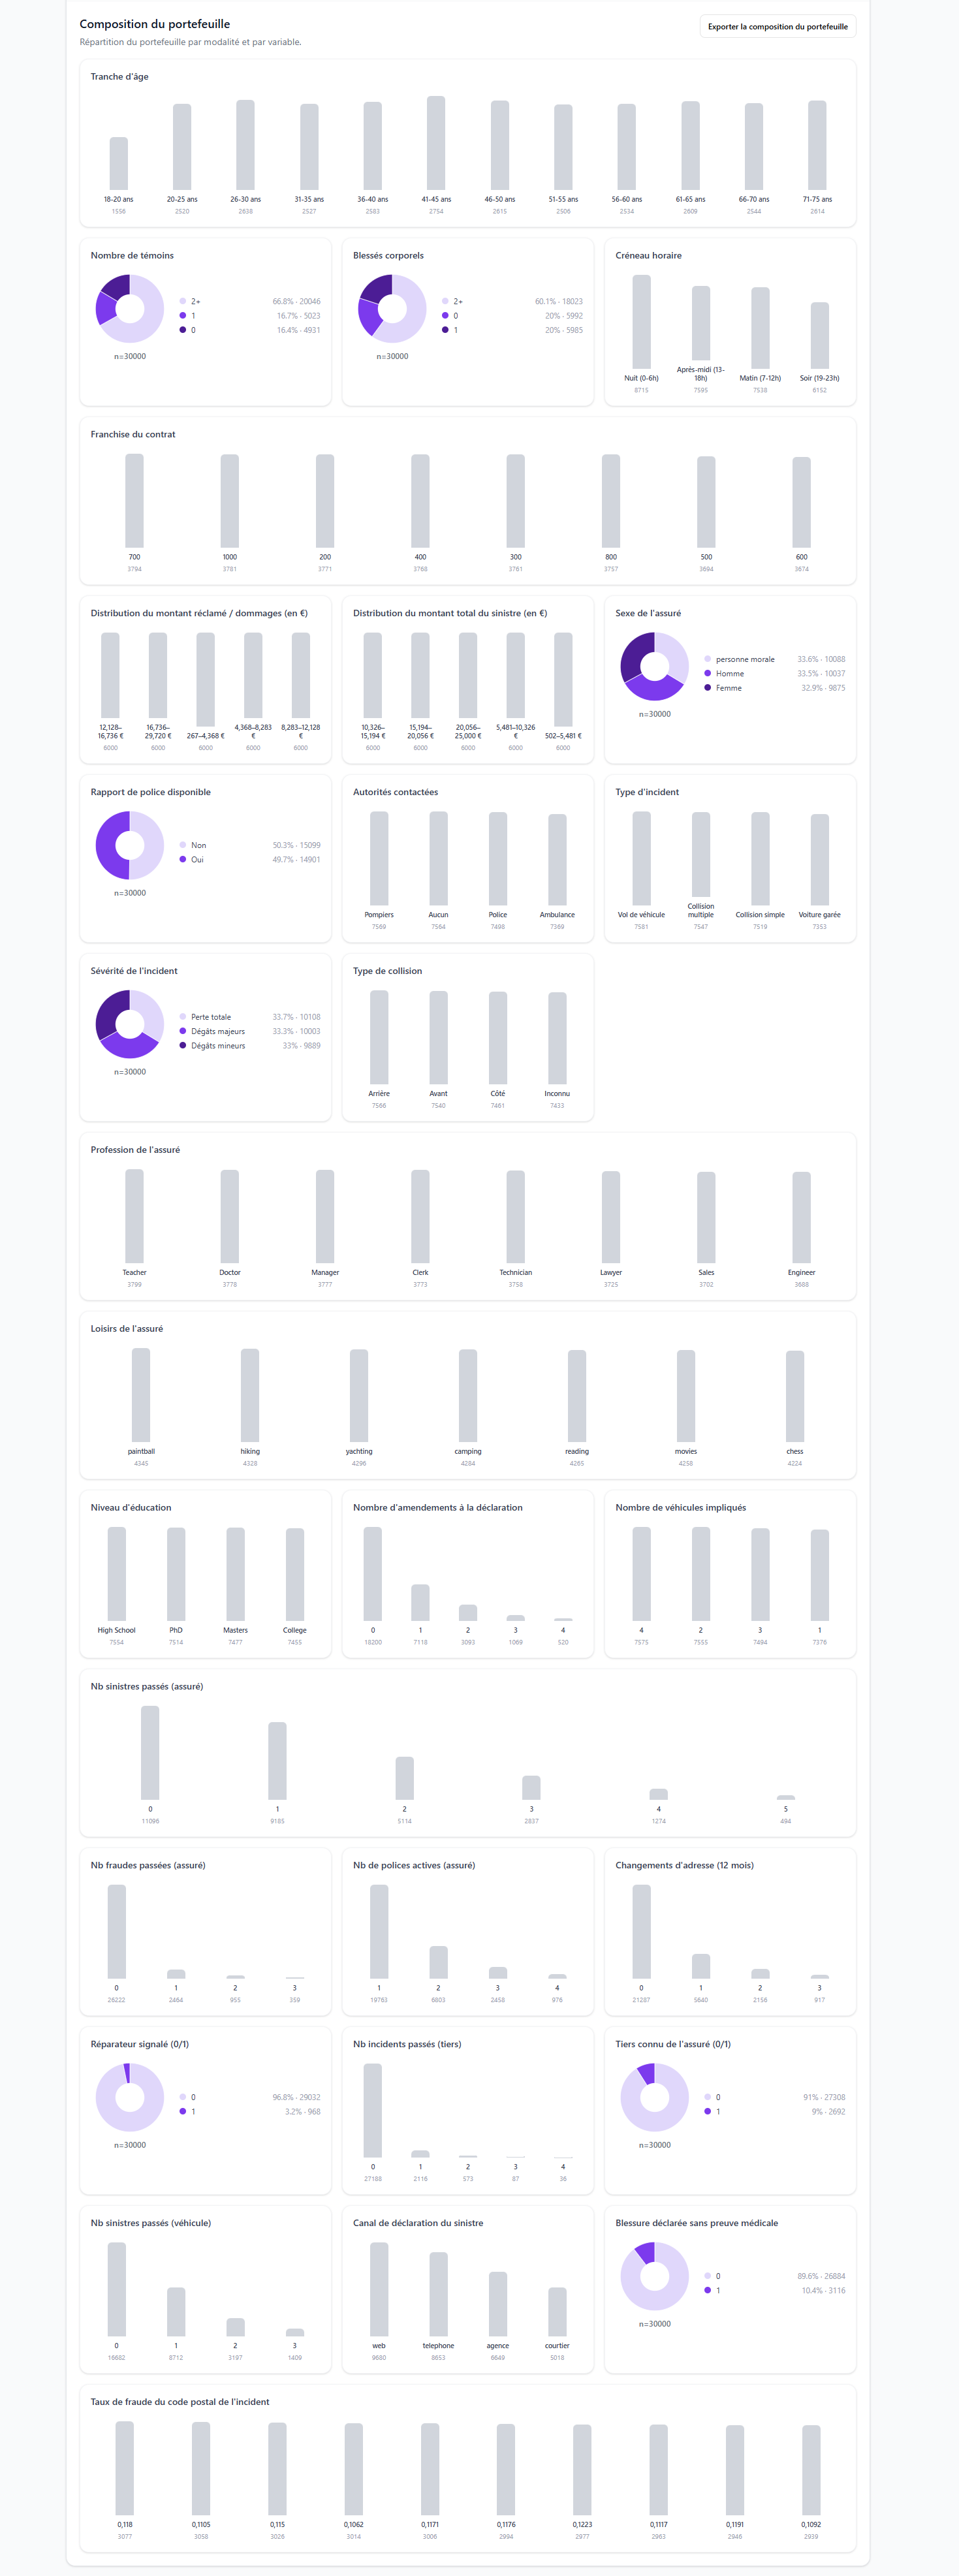
\includegraphics[width=\textwidth,height=0.85\textheight,keepaspectratio]{images/annexe/compo_portefeuille.png}
\end{center}